\documentclass[10pt]{article}
\usepackage{amsmath}
\usepackage{array}
\usepackage[legalpaper, margin=0.4in]{geometry}
\usepackage{graphicx} 

\title{Linear Optimization Set 1}
\author{Student Name: Erla Priyanka}
\date{Student ID: 1606063}
\begin{document}

\maketitle

\section*{Question 1. Blend Problem: Maximizing Profit for Motor Oil Production}

\subsection*{Objective}
Determine the optimal mix of components in each motor oil grade (Super, Premium, and Extra) to maximize profit.

\subsection*{Decision Variables}
Let:
\begin{itemize}
    \item \( x_{1S}, x_{2S}, x_{3S} \) = barrels of components 1, 2, and 3 used in Super grade, respectively.
    \item \( x_{1P}, x_{2P}, x_{3P} \) = barrels of components 1, 2, and 3 used in Premium grade, respectively.
    \item \( x_{1E}, x_{2E}, x_{3E} \) = barrels of components 1, 2, and 3 used in Extra grade, respectively.
\end{itemize}

\subsection*{Objective Function}
Maximize profit \( Z \):
\[
Z = [23(x_{1S} + x_{2S} + x_{3S}) + 20(x_{1P} + x_{2P} + x_{3P}) 
+ 18(x_{1E} + x_{2E} + x_{3E})] - [12(x_{1S} + x_{1P} + x_{1E}) 
+ 10(x_{2S} + x_{2P} + x_{2E}) + 14(x_{3S} + x_{3P} + x_{3E})]
\]

\subsection*{Constraints}

\begin{enumerate}
    \item \textbf{Component Availability:}
    \begin{align*}
    x_{1S} + x_{1P} + x_{1E} &\leq 4500 \\
    x_{2S} + x_{2P} + x_{2E} &\leq 2700 \\
    x_{3S} + x_{3P} + x_{3E} &\leq 3500
    \end{align*}
    
    \item \textbf{Grade Specifications:}
    \begin{itemize}
        \item \textbf{Super:}
        \begin{align*}
        x_{1S} &\geq 0.5(x_{1S} + x_{2S} + x_{3S}) \\
        x_{2S} &\leq 0.3(x_{1S} + x_{2S} + x_{3S})
        \end{align*}
        \item \textbf{Premium:}
        \begin{align*}
        x_{1P} &\geq 0.4(x_{1P} + x_{2P} + x_{3P}) \\
        x_{3P} &\leq 0.25(x_{1P} + x_{2P} + x_{3P})
        \end{align*}
        \item \textbf{Extra:}
        \begin{align*}
        x_{1E} &\geq 0.6(x_{1E} + x_{2E} + x_{3E}) \\
        x_{2E} &\geq 0.1(x_{1E} + x_{2E} + x_{3E})
        \end{align*}
    \end{itemize}
    
    \item \textbf{Production Limits:}
    \begin{align*}
    x_{1S} + x_{2S} + x_{3S} &\leq 3000 \\
    x_{1P} + x_{2P} + x_{3P} &\leq 3000 \\
    x_{1E} + x_{2E} + x_{3E} &\leq 3000
    \end{align*}
\end{enumerate}

\subsection*{Methodology}

\begin{enumerate}
    \item \textbf{Formulate the Linear Program:}
    \begin{itemize}
        \item Objective Function: \( Z \)
        \item Constraints: Component Availability, Grade Specifications, Production Limits
    \end{itemize}
    
    \item \textbf{Use a Solver:}
    \begin{itemize}
        \item Apply optimization using Excel Solver
       
    \end{itemize}
\end{enumerate}

\subsection*{Solution}
Optimal Mix (in barrels per day):

\begin{tabular}{|c|c|c|c|}
\hline
Grade & Component 1 & Component 2 & Component 3 \\
\hline
Super & 1700 & 1000 & 700 \\
Premium & 2200 & 0 & 800 \\
Extra & 500 & 1700 & 0 \\
\hline
\end{tabular}

\subsection*{Optimized Maximum Profit}
\$52,400 per day.
\vspace{290pt}
\begin{center}
    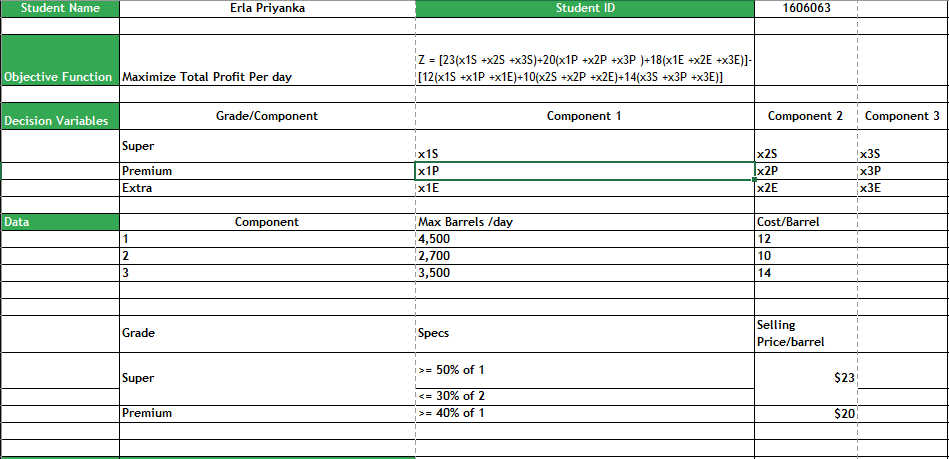
\includegraphics[width=\textwidth]{https://github.com/theyardmic/ETH-bank/blob/bce4280e4e0ac3d00c1704f11f021a11b0eea7ca/Q1.PNG} % Adjust the width as needed
\end{center}
\newpage


\section*{Question 2. Make or Buy Problem: Maximizing Profit for HDD and SSD Production}

\subsection*{Objective}
Determine the optimal number of Hard Disk Drives (HDD) and Solid State Drives (SSD) to fabricate in-house and purchase from a subcontractor to maximize profit.

\subsection*{Decision Variables}
Let:
\begin{itemize}
    \item \( x_{H,in} \) = Number of HDDs fabricated in-house.
    \item \( x_{S,in} \) = Number of SSDs fabricated in-house.
    \item \( x_{H,out} \) = Number of HDDs purchased from the subcontractor.
    \item \( x_{S,out} \) = Number of SSDs purchased from the subcontractor.
\end{itemize}

\subsection*{Objective Function}
Maximize profit \( Z \):
\[
Z = [(82 - 75)x_{H,in} + (125 - 117)x_{S,in} + (82 - 79)x_{H,out} + (125 - 123)x_{S,out}]
\]

\subsection*{Constraints}

\begin{enumerate}
    \item \textbf{Demand Satisfaction:}
    \begin{align*}
    x_{H,in} + x_{H,out} &\geq 2215 \text{ (HDD demand)} \\
    x_{S,in} + x_{S,out} &\geq 1512 \text{ (SSD demand)} \\
    x_{H,in} + x_{S,in} &\leq 2282 \text{ (Total HDD+SSD production limit)}
    \end{align*}
    
    \item \textbf{Production Capacity:}
    \begin{align*}
    0.1x_{H,in} + 0.12x_{S,in} &\leq 350 \text{ (Fabrication)} \\
    0.15x_{H,in} + 0.11x_{S,in} &\leq 230 \text{ (Assembly)} \\
    0.13x_{H,in} + 0.13x_{S,in} &\leq 450 \text{ (Shipping)}
    \end{align*}
\end{enumerate}

\subsection*{Methodology}

\begin{enumerate}
    \item \textbf{Formulate the Linear Program:}
    \begin{itemize}
        \item Objective Function: \( Z \)
        \item Constraints: Demand Satisfaction, Production Capacity
    \end{itemize}
    
    \item \textbf{Use a Linear Optimizer:}
    \begin{itemize}
        \item Apply Excel Solver  to determine the optimal values for \( x_{H,in}, x_{S,in}, x_{H,out}, x_{S,out} \).
    \end{itemize}
\end{enumerate}

\subsection*{Solution}
Optimal Production (units per month):

\begin{tabular}{|c|c|c|}
\hline
 & HDD & SSD \\
\hline
In-house & 424.53 & 1512 \\
Subcontracted & 345.47 & 0 \\
\hline
\end{tabular}

\subsection*{Maximum Profit}
\$16,104.13 per month.
\newpage
\begin{center}
    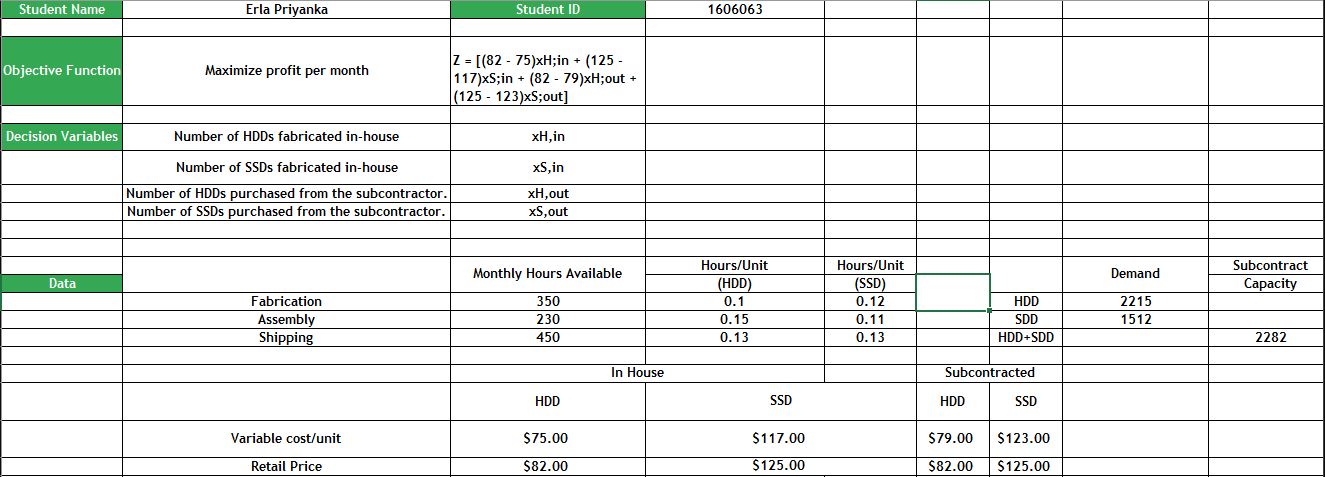
\includegraphics[width=\textwidth]{https://github.com/theyardmic/ETH-bank/blob/bce4280e4e0ac3d00c1704f11f021a11b0eea7ca/Q2.PNG} % Adjust the width as needed
\end{center} % Fills the space until halfway down the page

\end{document}
